%%%%%%%%%%%%%%%%%%%%%%%%%%%%%%%%%%%%%%%%%%%%%%%%%%%
%
%  New template code for TAMU Theses and Dissertations starting Fall 2016.
%
%
%  Original Author: Sean Zachary Roberson
%  This version adapted for URS by Parasol lab.
%  Adapted from version 3.16.10, which was last updated on 9/29/2016.
%  URS adaptation last updated 1/9/2017.
%
%%%%%%%%%%%%%%%%%%%%%%%%%%%%%%%%%%%%%%%%%%%%%%%%%%%
%%%%%%%%%%%%%%%%%%%%%%%%%%%%%%%%%%%%%%%%%%%%%%%%%%%%%%%%%%%%%%%%%%%%%%
%%                           INTRODUCTION
%%%%%%%%%%%%%%%%%%%%%%%%%%%%%%%%%%%%%%%%%%%%%%%%%%%%%%%%%%%%%%%%%%%%%


\pagestyle{plain} % No headers, just page numbers
%\pagenumbering{arabic} % Arabic numerals
%\setcounter{page}{1}

\chapter{INTRODUCTION}

\section{Background}

Textbooks go through a long and arduous process before a student or professor is able to view and use it. This process requires much work and effort into not only validating the content of the textbook but also validating the ordering of the textbook as whole. Much like a jigsaw puzzle, each chapter fits one after another based on the dependency of the topics being taught. On top of these chapters being ordered, the exercises must also be placed in the correct place in order to not give an exercise that is based on a topic that has not been presented to the reader previously.

After all this work on ordering has been completed (among other meticulous things), the textbook is finally ready for publication. As with many good textbooks, many professors and institutions may enjoy the content within the textbook but would prefer delivering the content to a student in a different order than the current order of the textbook. Most of the time, the work and effort that has gone into meticulously ordering the chapters and exercises must now be revisited again and modified. This process is nearly as time consuming and laborious as the first going through this process and is frequently done imperfectly.

\section{Resulting Platform}

In order to achieve a desired solution, a full stack web application was built. The integration points from the textbook to the application consists of five networks. In the current version of the platform, uploading three of the networks into the platform is all that is required for the structures and dependencies of any given textbook to be fully understood and used Fig \ref{fig:textbooks}. After transforming these networks into a directed acyclic graph that is then stored into the graph database, a figure can be generated as is show for units in Fig \ref{fig:graph}.

\begin{figure}[ht]
    \centering
    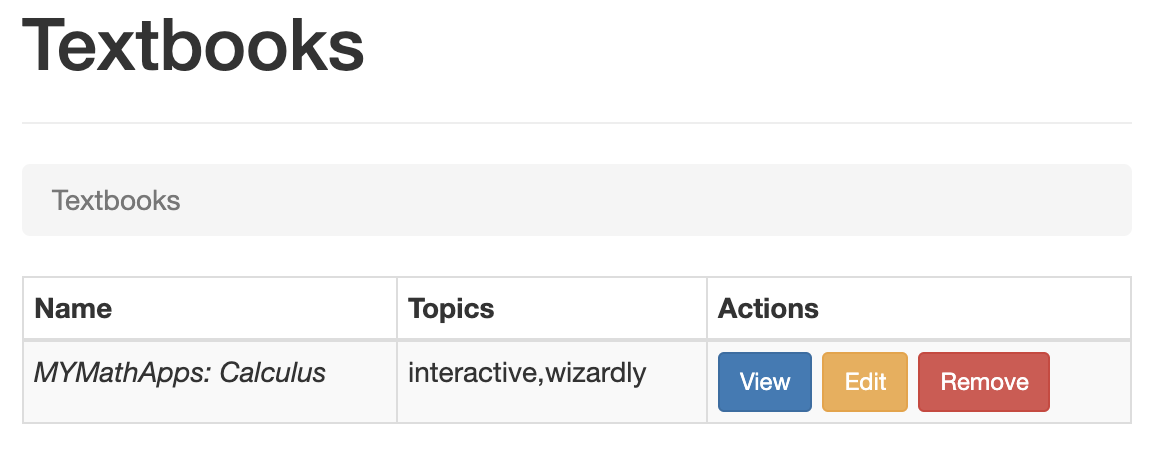
\includegraphics[scale=0.5]{textbooks.png}
    \caption[Textbook selection.]{The selection and upload of networks for a given textbook}
        
    \label{fig:textbooks}
\end{figure}

\begin{figure}[ht]
    \centering
    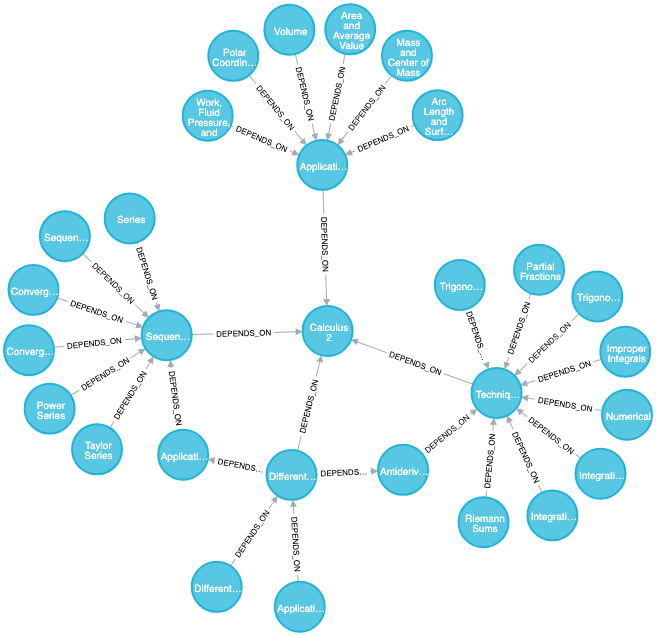
\includegraphics[scale=0.5]{graph.png}
    \caption[Textbook selection.]{The selection and upload of networks for a given textbook}
        
    \label{fig:graph}
\end{figure}


The second piece of the platform a interactive graphical table of contents where the units can be dragged around to reorder them Fig \ref{fig:nestedChapters}. It the actual piece of the platform that allows an editor to reorder and restructure the original ordering of the textbook. Each unit and sub unit can be toggled to view more or less about units. There is also a button to toggle all units to be viewed or to collapse all units until only the independent root units are viewable.

\begin{figure}[ht]
    \centering
    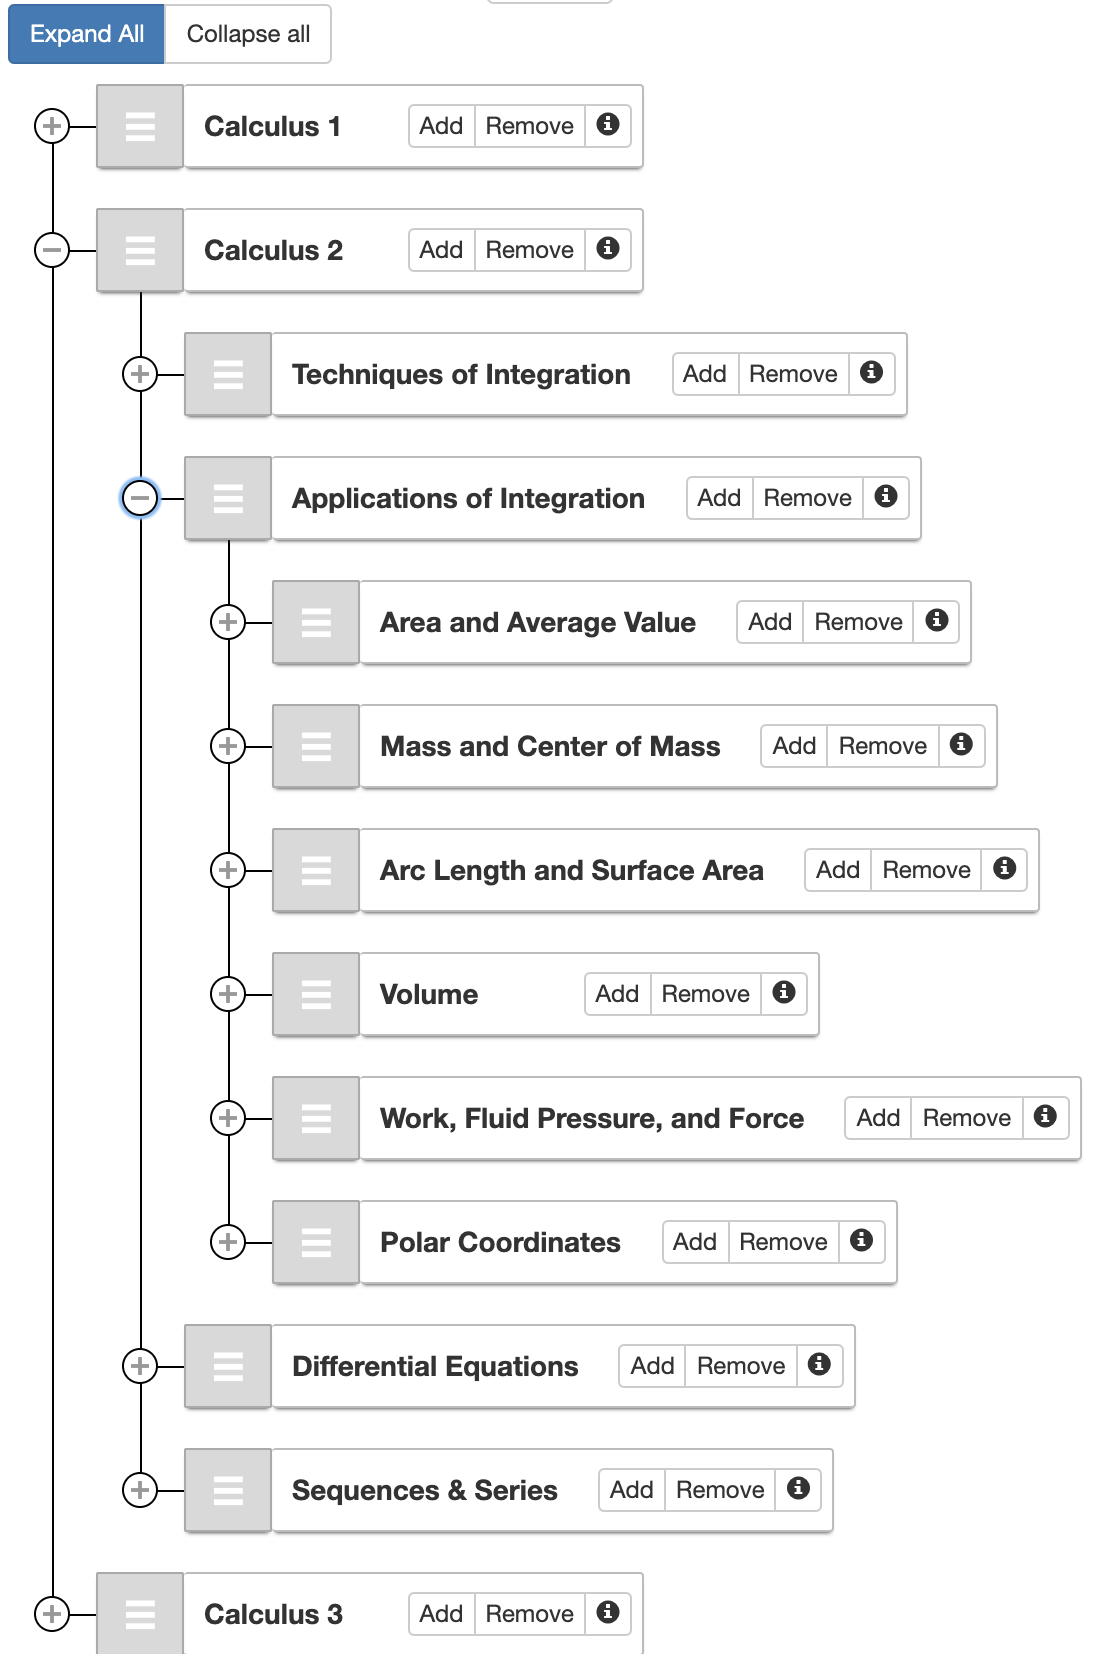
\includegraphics[scale=0.3]{nestedChapters.png}
    \caption[Unit hierarchy.]{Unit hierarchy.}
        
    \label{fig:nestedChapters}
\end{figure}

\pagebreak

On top of being toggleable, each unit is draggable Fig \ref{fig:chaptersMoving}. This allows for each unit to be moved to any other point in the structure of the tree or table of contents. During each of these movements, a request is sent to the server to verify that all dependencies are met. If any dependency is not met, a message is then sent to the front end for it to be displayed to the user.

\begin{figure}[ht]
    \centering
    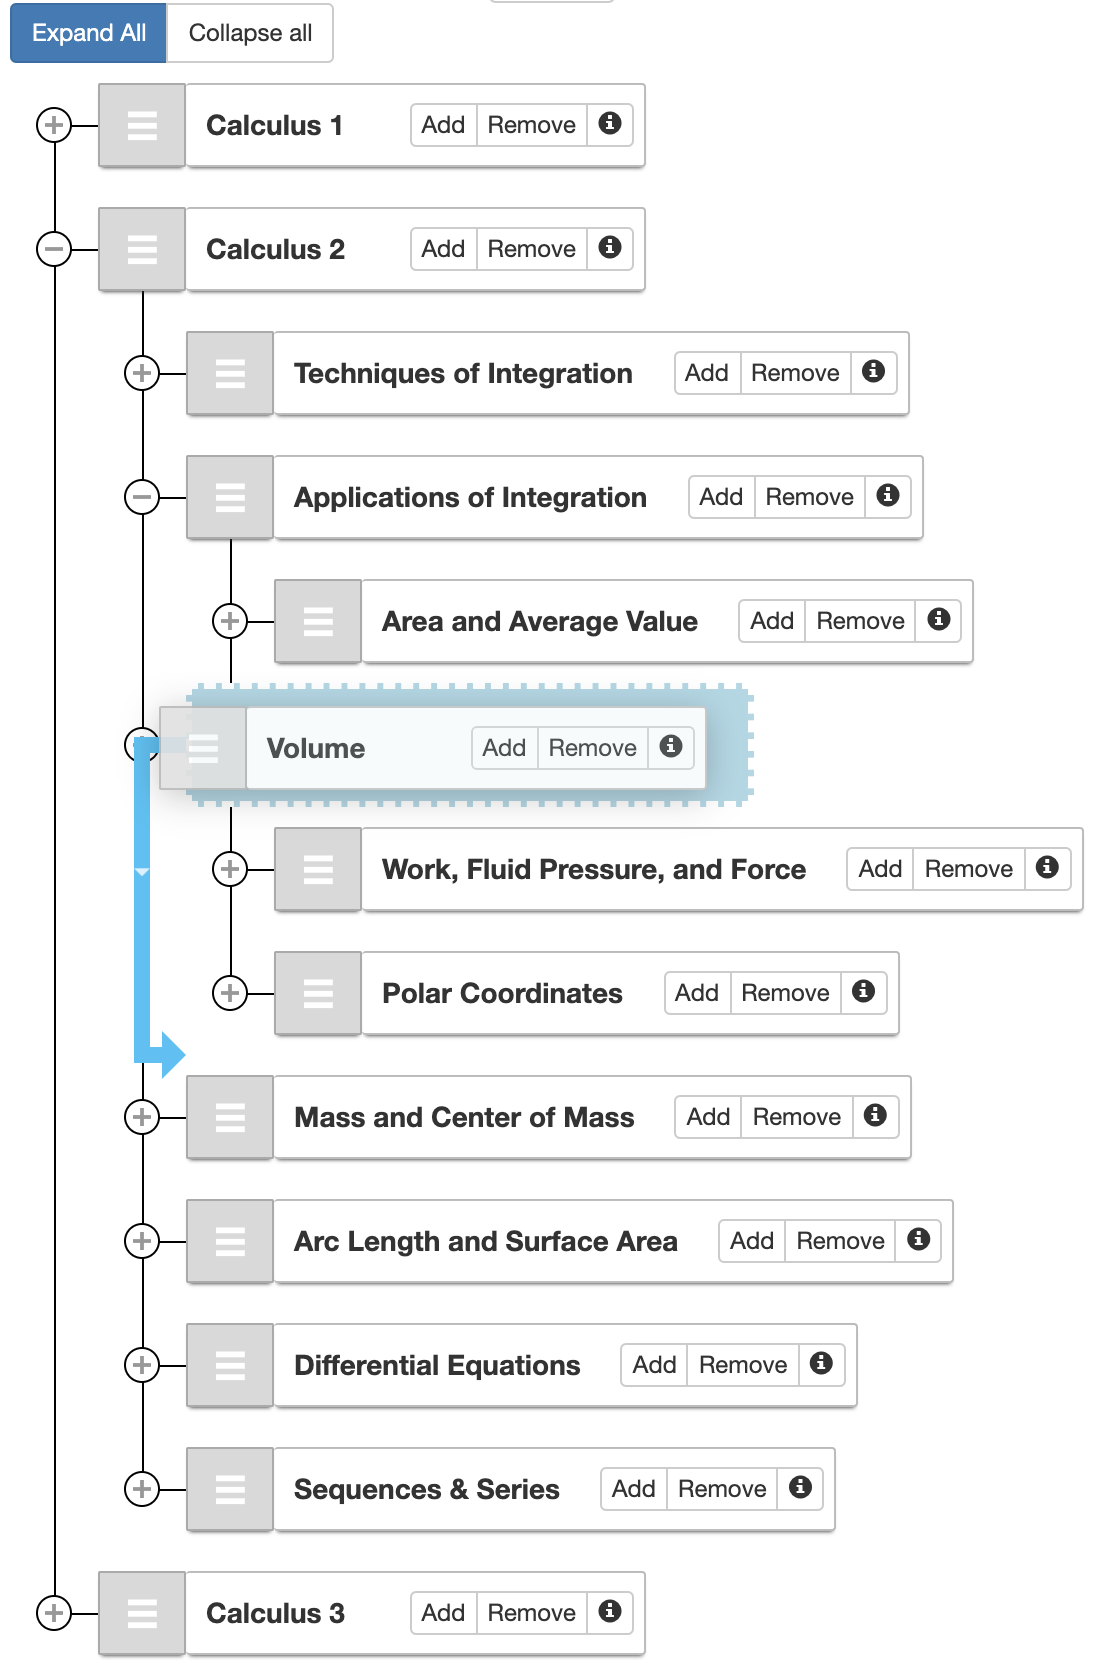
\includegraphics[scale=0.3]{chaptersMoving.png}
    \caption[Reordering units.]{Reordering of units through the use of dragging.}
        
    \label{fig:chaptersMoving}
\end{figure}

\pagebreak
